\title{Perry Williams}
\author{Ecologist and Statistician \\ Associate Professor \\ Department of Natural Resources and Environmental Science \\ University of Nevada, Reno}
\date{\today}


\maketitle

\begin{center}
  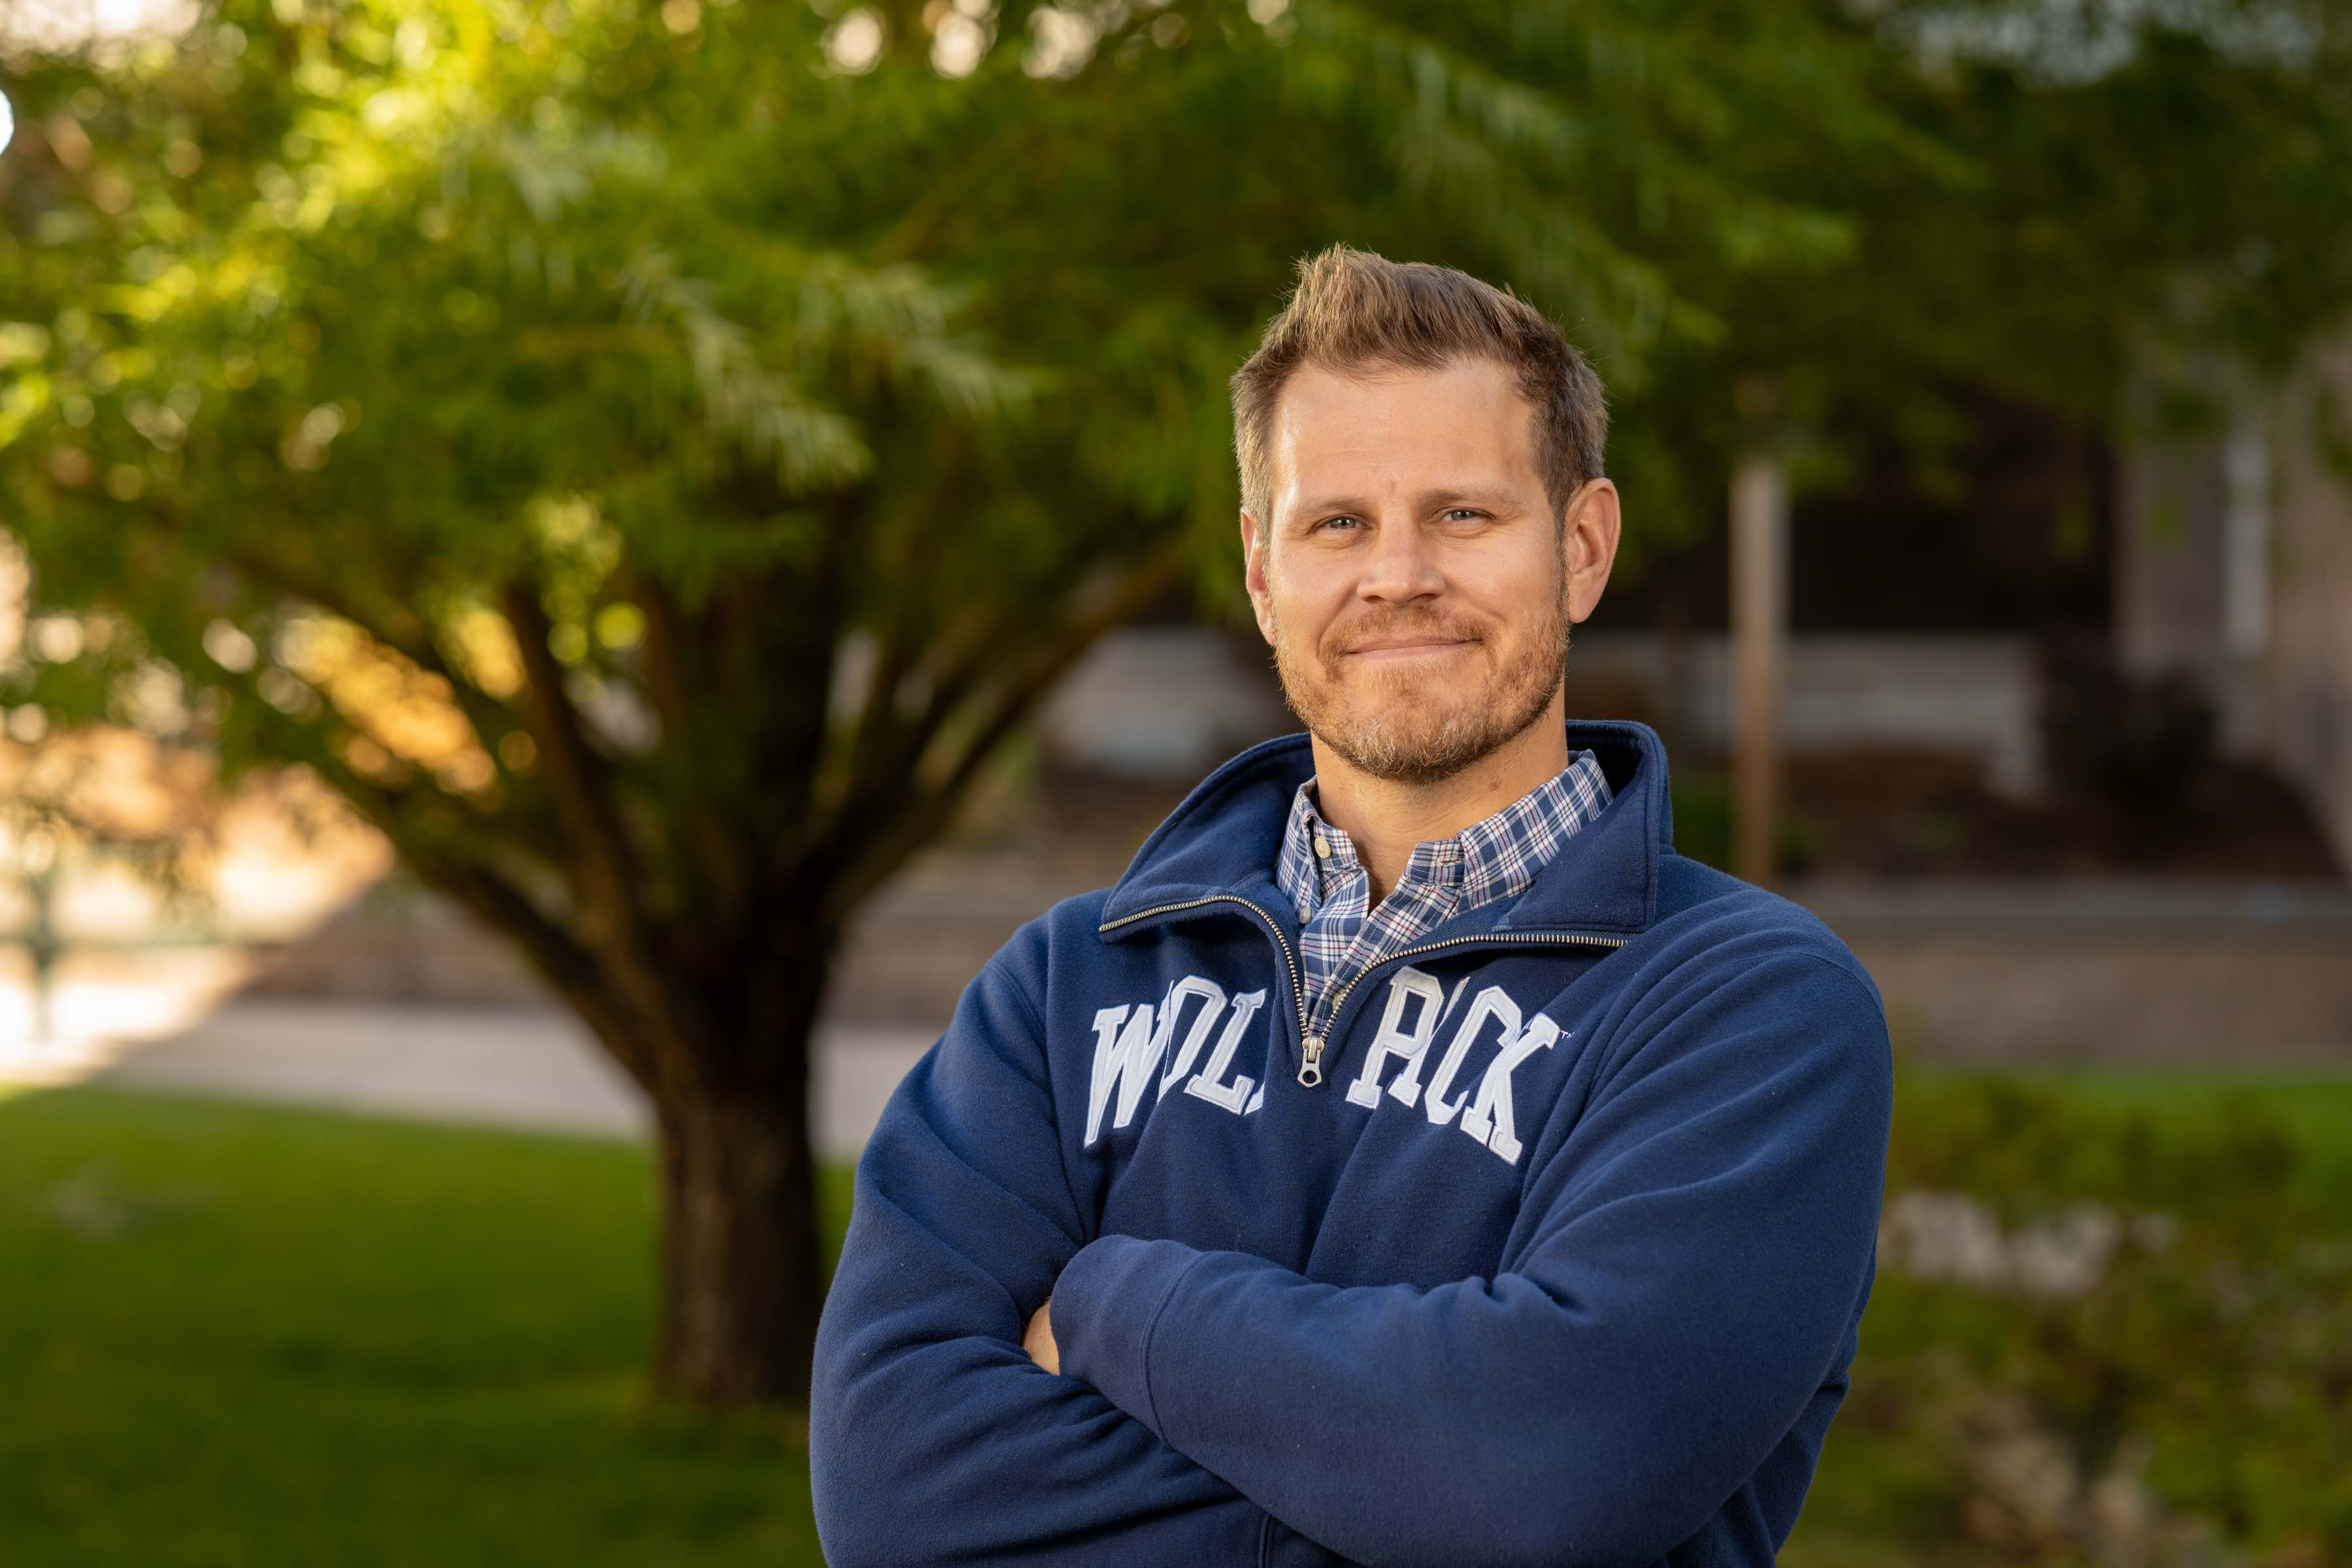
\includegraphics[width=0.35\textwidth]{assets/perry_2024.jpg}
\end{center}

\section*{About Me}
I am an Associate Professor in the Department of Natural Resources and Environmental Science at the University of Nevada, Reno.  
My work explores how populations and ecosystems change across space and time, with an emphasis on discovery and understanding of complex natural processes.  
I develop statistical and computational tools that advance ecological science, improve our ability to forecast environmental dynamics, and deepen knowledge of the natural world.


\section*{Contact}
\begin{itemize}
  \item Email: \href{mailto:perryw@unr.edu}{perryw@unr.edu}
  \item GitHub: \url{https://github.com/perrywilliamsunr}
  \item Google Scholar · ORCID
\end{itemize}

\section*{Current Projects}
\begin{itemize}
  \item \textbf{EcoDiffusion}: developing an R package for hierarchical Bayesian ecological diffusion models that help reveal how populations and processes spread across landscapes.
  \item Investigating population dynamics and movement in species such as sage grouse to understand large-scale patterns of ecological change.
  \item Exploring how human activities and natural variation shape the distribution of species, using case studies that include sea otters and other wildlife populations.
\end{itemize}

